\section{Oxygen}

\begin{multicols}{2}


\section*{Preparation of Oxygen}


\subsection{Using Hydrogen Peroxide}

%\begin{center}
%\includegraphics[width=0.4\textwidth]{./img/.png}
%\end{center}

\begin{description*}
%\item[Subtopic:]{}
\item[Materials:]{Dry cell, hydrogen peroxide, water, plastic bottle}
\item[Setup:]{Open a dry cell battery and peel back the metal casing to reveal a black powder. This is Manganese (IV) oxide. }
\item[Procedure:]{Scoop out the powder and place in a plastic bottle. Add about 20 mL of dilute hydrogen peroxide. Crush and cap the bottle.}
\item[Hazards:]{Hydrogen peroxide is corrosive. Be sure to dilute the solution.}
%\item[Questions:]{}
\item[Observations:]{The bottle inflates with oxygen gas.}
\item[Theory:]{Hydrogen peroxide decomposes into water and oxygen rather easily. The manganese (IV) dioxide acts as a catalyst. The chemical equation for this reaction is: \[ 2\mathrm{H}_2\mathrm{O}_2 + ( \mathrm{Mn}\mathrm{O}_2 ) \longrightarrow 2\mathrm{H}_2\mathrm{O} + \mathrm{O}_2 \]}
%\item[Applications:]{}
%\item[Notes:]{}
\end{description*}

\subsection{Using A Yeast Catalyst} % Shika 229

%\begin{center}
%\includegraphics[width=0.4\textwidth]{./img/.jpg}
%\end{center}

\begin{description*}
%\item[Subtopic:]{}
\item[Materials:]{Hydrogen peroxide, water, yeast, plastic bottle}
%\item[Setup:]{}
\item[Procedure:]{Place a small amount of dilute hydrogen peroxide in a plastic bottle. Crush the bottle and add some yeast. Cap the bottle and gently invert.}
%\item[Hazards:]{}
%\item[Questions:]{}
%\item[Observations:]{}
\item[Theory:]{Yeast contains an enzyme called catalase, which helps to break down hydrogen peroxide into oxygen and water. The enzyme protects the organism by eating the peroxide.}
%\item[Applications:]{}
%\item[Notes:]{}
\end{description*}

\subsection{Elephant Toothpaste} % PIC!!!

%\begin{center}
%\includegraphics[width=0.4\textwidth]{./img/.jpg}
%\end{center}

\begin{description*}
%\item[Subtopic:]{}
\item[Materials:]{Syringe/measuring cylinder, powdered soap, yeast, hydrogen peroxide, food colour}
%\item[Setup:]{}
\item[Procedure:]{Mix powdered soap and a warm yeast solution in a syringe or large measuring cylinder. Add food colouring if desired. Pour in hydrogen peroxide.}
%\item[Hazards:]{}
%\item[Questions:]{}
\item[Observations:]{A large amount of foam/bubbles bursts out of the container.}
\item[Theory:]{Catalase decomposes hydrogen peroxide to form water and oxygen
gas. The soap
traps the gas in bubbles. These bubbles build up upon each other, slowly
forcing them out of the container. }
%\item[Applications:]{}
%\item[Notes:]{}
\end{description*}

\vfill
\columnbreak

\subsection{Using Potassium Manganate (VII)} % Shika 282

\begin{center}
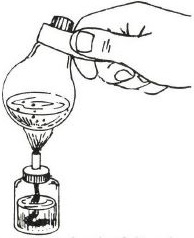
\includegraphics[width=0.25\textwidth]{./img/source/oxygen-prep.jpg}
\end{center}

\begin{description*}
%\item[Subtopic:]{}
\item[Materials:]{Potassium manganate (VII), \nameref{sec:heatsources}, test tube/light bulb}
%\item[Setup:]{}
\item[Procedure:]{Carefully heat potassium manganate (VII) (permanganate) in a test
tube or in an opened electric bulb.}
%\item[Hazards:]{}
%\item[Questions:]{}
%\item[Observations:]{}
\item[Theory:]{Chemical equation for this reaction: \[ 2\mathrm{K}\mathrm{Mn}\mathrm{O}_4 \longrightarrow \mathrm{K}_2\mathrm{Mn}\mathrm{O}_4 + \mathrm{Mn}\mathrm{O}_2 + \mathrm{O}_2 \]}
%\item[Applications:]{}
%\item[Notes:]{}
\end{description*}

%==================================================================================================%

\section*{Properties of Oxygen}


\subsection{Burning in Pure Oxygen}

\begin{center}
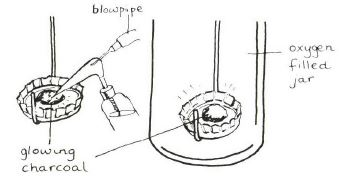
\includegraphics[width=0.4\textwidth]{./img/source/burning-oxygen.jpg}
\end{center}

\begin{description*}
%\item[Subtopic:]{}
\item[Materials:]{Charcoal, deflagrating spoon, straw, bottle}
%\item[Setup:]{}
\item[Procedure:]{(a) Ignite charcoal in a deflagrating spoon
using a blow pipe. Then put the deflagrating
spoon with the burning charcoal into a glass full
of pure oxygen.

(b) Bring glowing iron wool into a glass full of
pure oxygen.}
%\item[Hazards:]{}
%\item[Questions:]{}
\item[Observations:]{Both substances bum with bright flame.}
\item[Theory:]{Charcoal forms carbon dioxide and iron
forms iron oxide. Both reactions give out heat
(exothermic reactions).}
%\item[Applications:]{}
%\item[Notes:]{}
\end{description*}

%==================================================================================================%


\end{multicols}

\pagebreak